%%%%%%%%%%%%%%%%%%%%%%%%%%%%%%%%%%%%%%%%%%%%%%%%%%%%%%%%%%%%%%%%%%%%%%%%%%%%%%%%%%%%%%%%%%%%%%%%
%
% CSCI 1290 final writeup
%
%%%%%%%%%%%%%%%%%%%%%%%%%%%%%%%%%%%%%%%%%%%%%%%%%%%%%%%%%%%%%%%%%%%%%%%%%%%%%%%%%%%%%%%%%%%%%%%%

\documentclass[11pt]{article}

\usepackage[english]{babel}
\usepackage[utf8]{inputenc}
\usepackage[colorlinks = true,
            linkcolor = blue,
            urlcolor  = blue]{hyperref}
\usepackage[a4paper,margin=0.75in]{geometry}
\usepackage{stackengine,graphicx}
\usepackage{fancyhdr}
\setlength{\headheight}{15pt}
\usepackage{microtype}
\usepackage{times}
\usepackage{booktabs}
\usepackage{subcaption} % for subfigures
\usepackage{enumitem} % extra package for no spacing between lists
\usepackage{amsmath} % extra package for aligned equations
\usepackage{amssymb} % extra pachage for real number and other symbols
\usepackage{listings} % for code blocks

\frenchspacing
\setlength{\parindent}{0cm} % Default is 15pt.
\setlength{\parskip}{0.3cm plus1mm minus1mm}

\pagestyle{fancy}
\fancyhf{}
\lhead{Final Project}
\rhead{CSCI 1290}
\rfoot{\thepage}

% objects for maketitle
\author{}
\date{2020.12.11}
\title{\vspace{-1cm}Patches Project}

\begin{document}
\maketitle
\vspace{-2cm}
\thispagestyle{fancy}

\subsection*{Project goal}

I started my project by aiming to utilise the fourier transform to create
blurs in an image. I was able to do this by transforming the image into the
fourier transform, multiplying it by a gaussian mask in the same space, then
taking the inverse fourier transform to have a blurred image. Once that was
done, I wanted to also use the fourier
transform to deblur an image. However I learned that deblurring an image
with the fourier transform is difficult without knowing what the mask
used was. Thus, at the suggestion of the professor, I partnered with
the blur-de-blur team who's main focus was on this specific question.

Below is a pristine image I used for reference and patches of blur within it
(I took it while in Japan in a city outside Kyoto at the beginning of the year
on a sony alpha-6000, a trip I have fond memories of now).

\begin{figure}[!ht]
  \centering
  \begin{subfigure}[b]{0.45\textwidth}
    \centering
    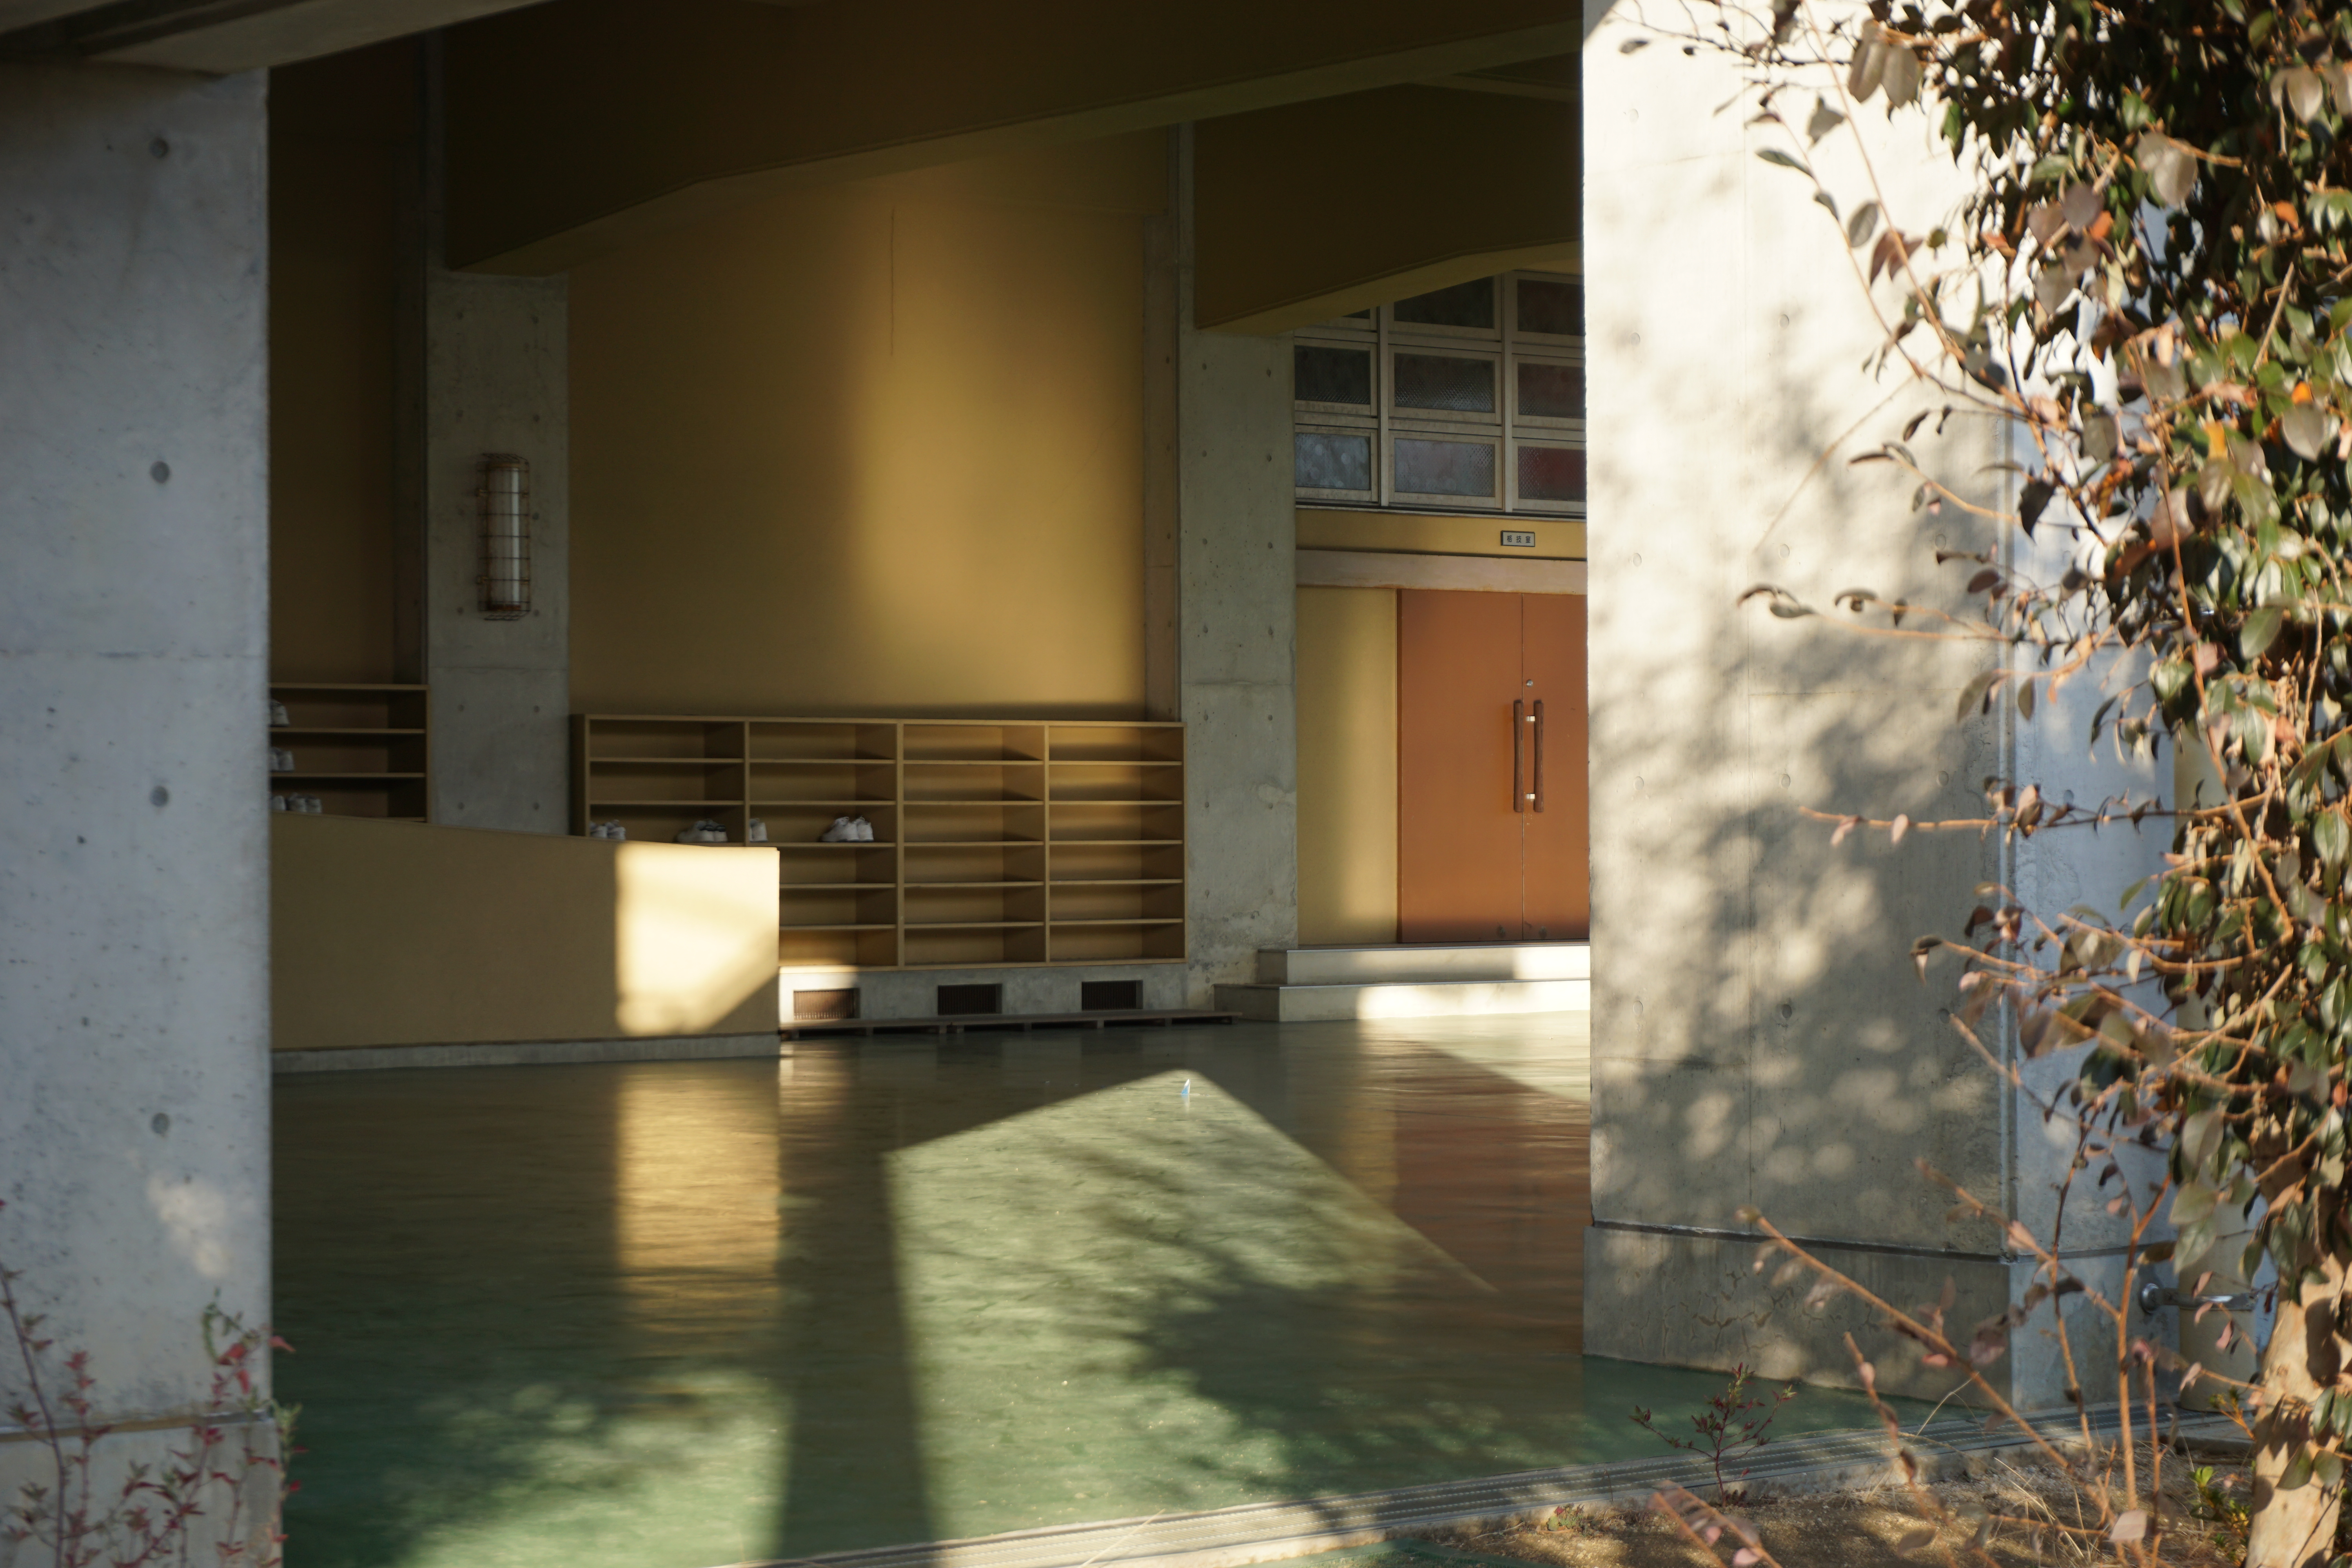
\includegraphics[width=1.0\textwidth]{pres_images/img01-original.JPG}
    \caption{pristine image}
  \end{subfigure}
  \hfill
  \begin{subfigure}[b]{0.45\textwidth}
    \centering
    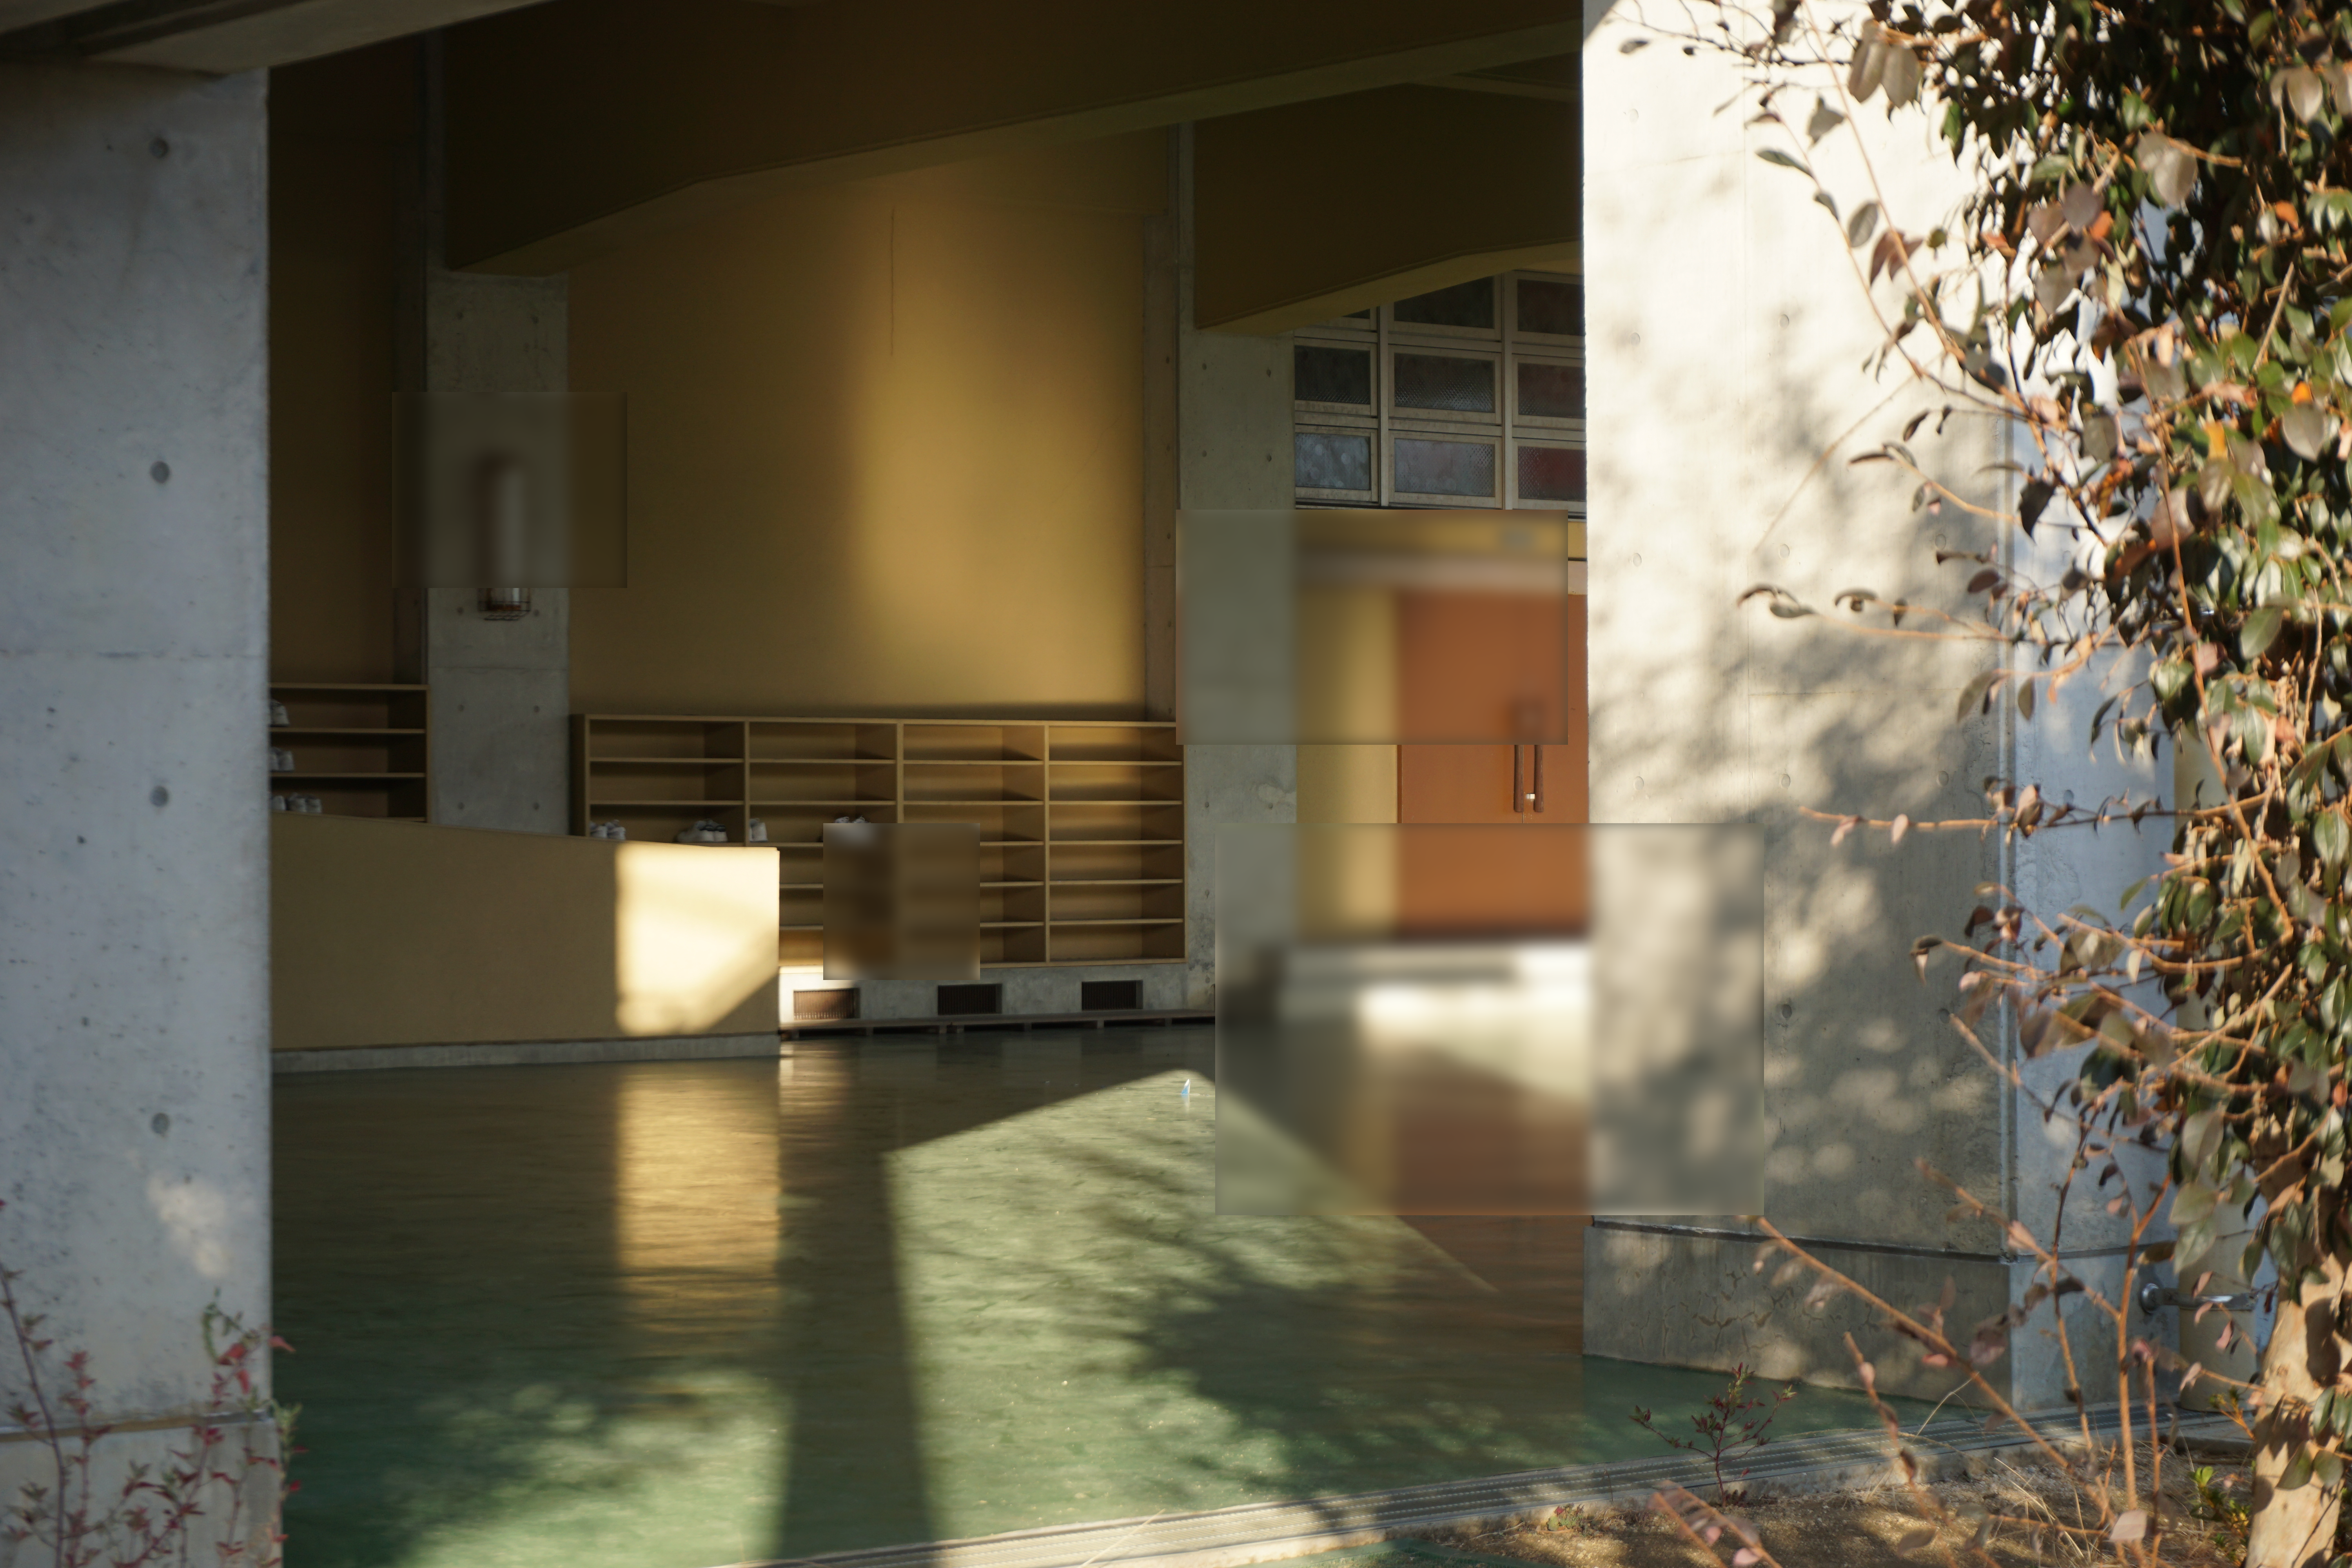
\includegraphics[width=1.0\textwidth]{pres_images/img02-blurred.png}
    \caption{blurred patches in image}
  \end{subfigure}
  
  \caption{}
  \label{fig:1}
\end{figure}


I wanted to expand my project. I sought to create patches of blur in an image,
locate the blur, apply the deblur algorithm, and insert it back into the image.
Straight forward enough, however some non-trivial questions arose:

\begin{itemize}
    \item How can one one classify an image as blurred? 
    \item How can one locate a blur in an image?
    \item In what assortment of ways can one best deblur a region?
\end{itemize}

This second question proved quite exciting to me. Before I answer
them let me go into a bit more detail of my code framework.

\subsection*{method}

I defined two classes, one for an input image, and one for a rectangle.
This helped in a number of ways.  By using a class for the image, I was
able to access the image and portions in the image, as well as defined
functions that quickly operated on the image in an efficient manner, such
as saving the image to disk or applying a patch into it.  A rectangle class
proved quite efficient as a way to define the corners of a rectangle.
By simply instantiating a new rectangle, I could assert that the inputs
were within bounds of the image, as well as calculate the width, height,
and area of the rectangle. Additionally by defining a standard cover
rectangle of a fixed height, when I took a random point within the image,
I had an efficient way to create a new rectangle with the nice asserts
and computations just described. To compute a large number of patches
within the image, by simply passing in a cover rectangle and a number n,
I was able to quickly sample from the image within a region that was within
bounds, create a rectangle, and append it to a resulting array.

\subsection*{classify blur}

With code that was quite extensible I started on the first major question.
I found a pretty straight forward solution in calculating the laplacian
of an image and using its variance. the laplacian is the sum of the second order
derivatives in a 3 by 3 convolution for each pixel. This is useful to tell us
about the edges and motion in an image. Thus if the variance in an image
is large, then there are many edges and we might classify it as not blurry.
If the variance is small, then there are fewer edges and we might classify
it as blurry. However a few shortcomes arose. First, this fails on images
the naturally don't have many edges, such as scenic images (ones I typically
like to take). Second, there isn't an establish way to calculate the threshold
for variance, simply try different values until it seems to work. I wasn't
vary satisfied with this, it didn't seem robust enough. For example, if you
take a small enough slice of an image, the variance will be lower than expected.
this giving a false positive. I sought to remedy this in one way. By normalizing
the variance into the range (0,1), I hoped it might solve some of these issues.
However, when I took nine patches in the image where I knew what the truth should
be, I had a 5/9 correct classification rate. That is when the patch was blurry
or overlapped a mostly blurry region, did it classify blurry, or if the patch
was in a non-blurry region or overlapped mostly non-blurry region, did it classify
as not blurry. Not great, but good enough for my purposes. I also suspected it
was a rabbit whole that could likely be a project in itself,
I resolved to keep what I had.

\subsection*{samples to cover an image}

To begin with, I immediately recognized that we could define an upper and lower
bound on the number of samples to cover an image. For the examples, the
cover rectangle is 100 by 100 and the input image is 4000 by 6000.

\subsubsection*{lower bound}

In a lower bound, if each patch is a union disjoint (they all align next to each
other) overlayed on the image, then we have a minimum number of patches to cover
an image. This can be computed by calculating the area of the larger image and
dividing it by the area of the cover patch. In my example this would be as
few as 2,400 samples. This would be too optimistic I thought. As the
probability that if we sampled 2,400 times, they would all align in the way
described, seemed quite unlikely. 

\subsubsection*{upper bound}

In an upper bound, if each patch was one pixel offset from the previous patch
then we can be certain we will cover the image. Additionally if we used this
number for random samples, then we are almost guaranteed we will cover the image
and that a sampled patch will include a blurred region. We would need
$(m-x) * (n-y)$ where m by n are the height and width of the image and x by y
are the height and width of the cover patch. In my example this would be
23,010,000 samples. Quite large. I wondered if I could do better.


\subsubsection*{cover bound}

I'll start by saying probability is not my strong suite. After much reading on
different probability bounds, the one I settled on was to calculate a covering number.
A covering number are the number of sperical balls of a fixed size to completely cover
a given space, with overlaps allowed (external so that we know we cover over the edges
as well). In euclidean space $\mathbb{R}^m$ where
$K \subset \mathbb{R}^m$ are the set of vectors whose length (norm) is at most $k$
within a $d$-dimensional subspace and $r$ is the radius of our fixed ball, then there
is a convenient formula to calculate the covering number for $K$.

\[
 N^{ext}_{r} (K) \leq ( \frac{2k \sqrt{d}} {r} )^d
\]

Now with a bit of imagination, if we say the diagonal of our image is $k$ (the largest
vector within $K$), $d$ is most definitely 2, and $r$ is the diagonal of our cover
image divided by two (to get a radius), then we have everything we need to calculate
a covering number! In my example this becomes 83,200.

\subsection*{post process - region of blur}

If we are given a patch that is labelled blur, we are still not certain exactly within
it if a portion is blurred or not. With this in mind I considered two options.
The first is to do a real time update in the image, so that once a patch is classified
blurred, it should be fully deblurred and put back into the image so that if this
region is sampled again, it should be left alone. The second thought is that we could
take a bounding box perhaps twice the area of the cover patch used to label the patch
as blurred. Then take a random sample in here with a random number of times (likely only
one to four), deblur in each case then use a metric, perhaps the laplacian variance again
to see which performs best in deblurring this region. I chose the former as I wasn't
certain the latter would perform any better. Additionaly, One could simply make the
cover patch smaller so that with high probability it only contains pixels of one label.

\subsection*{results}

First lets look at how well deblurring patches worked. Unfortunately it appears deblurring
is still hard. I used non-final weights, so it's possible these results could be better.
Comparing the image on the left where black patches indicate regions that are deblurred
on the right, it's hard to see any difference. Comparing the sum of the difference
between two patch before and after, I can confirm the algorithm is doing something, it's
just hard to tell.

\begin{figure}[!ht]
  \centering
  \begin{subfigure}[b]{0.45\textwidth}
    \centering
    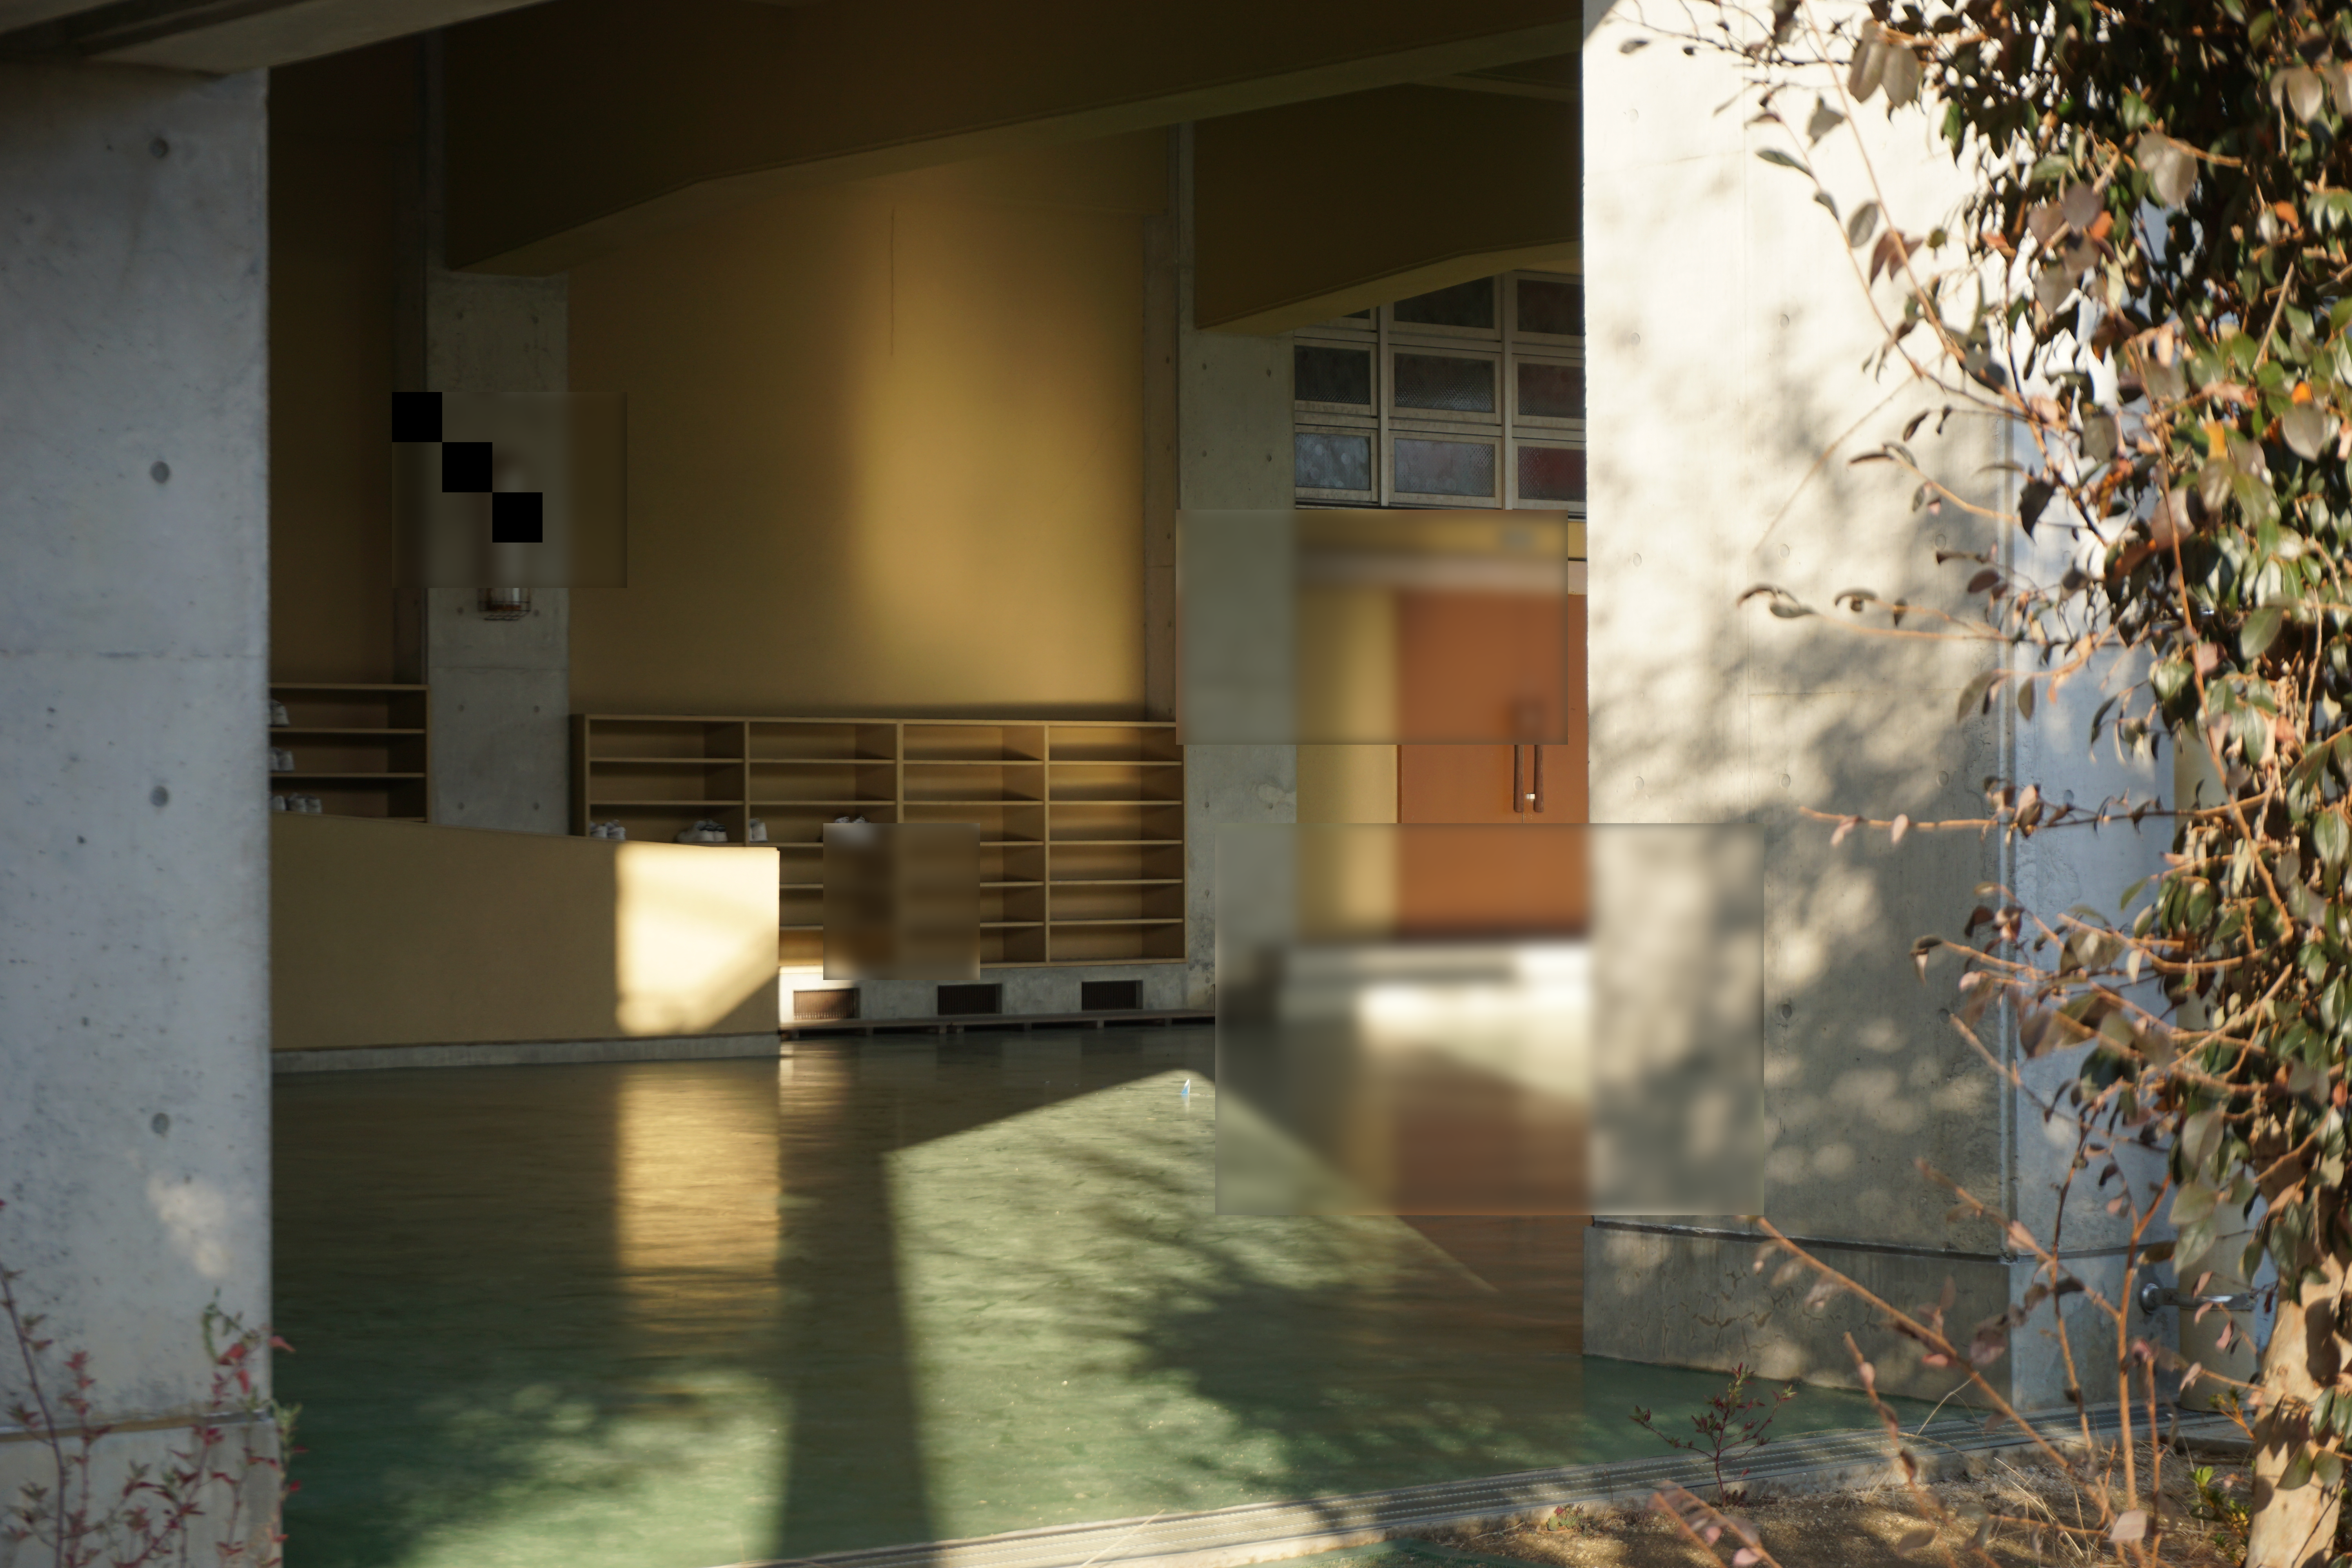
\includegraphics[width=1.0\textwidth]{pres_images/img04-de-blurred-blocks-test.png}
    \caption{patches for deblur}
  \end{subfigure}
  \hfill
  \begin{subfigure}[b]{0.45\textwidth}
    \centering
    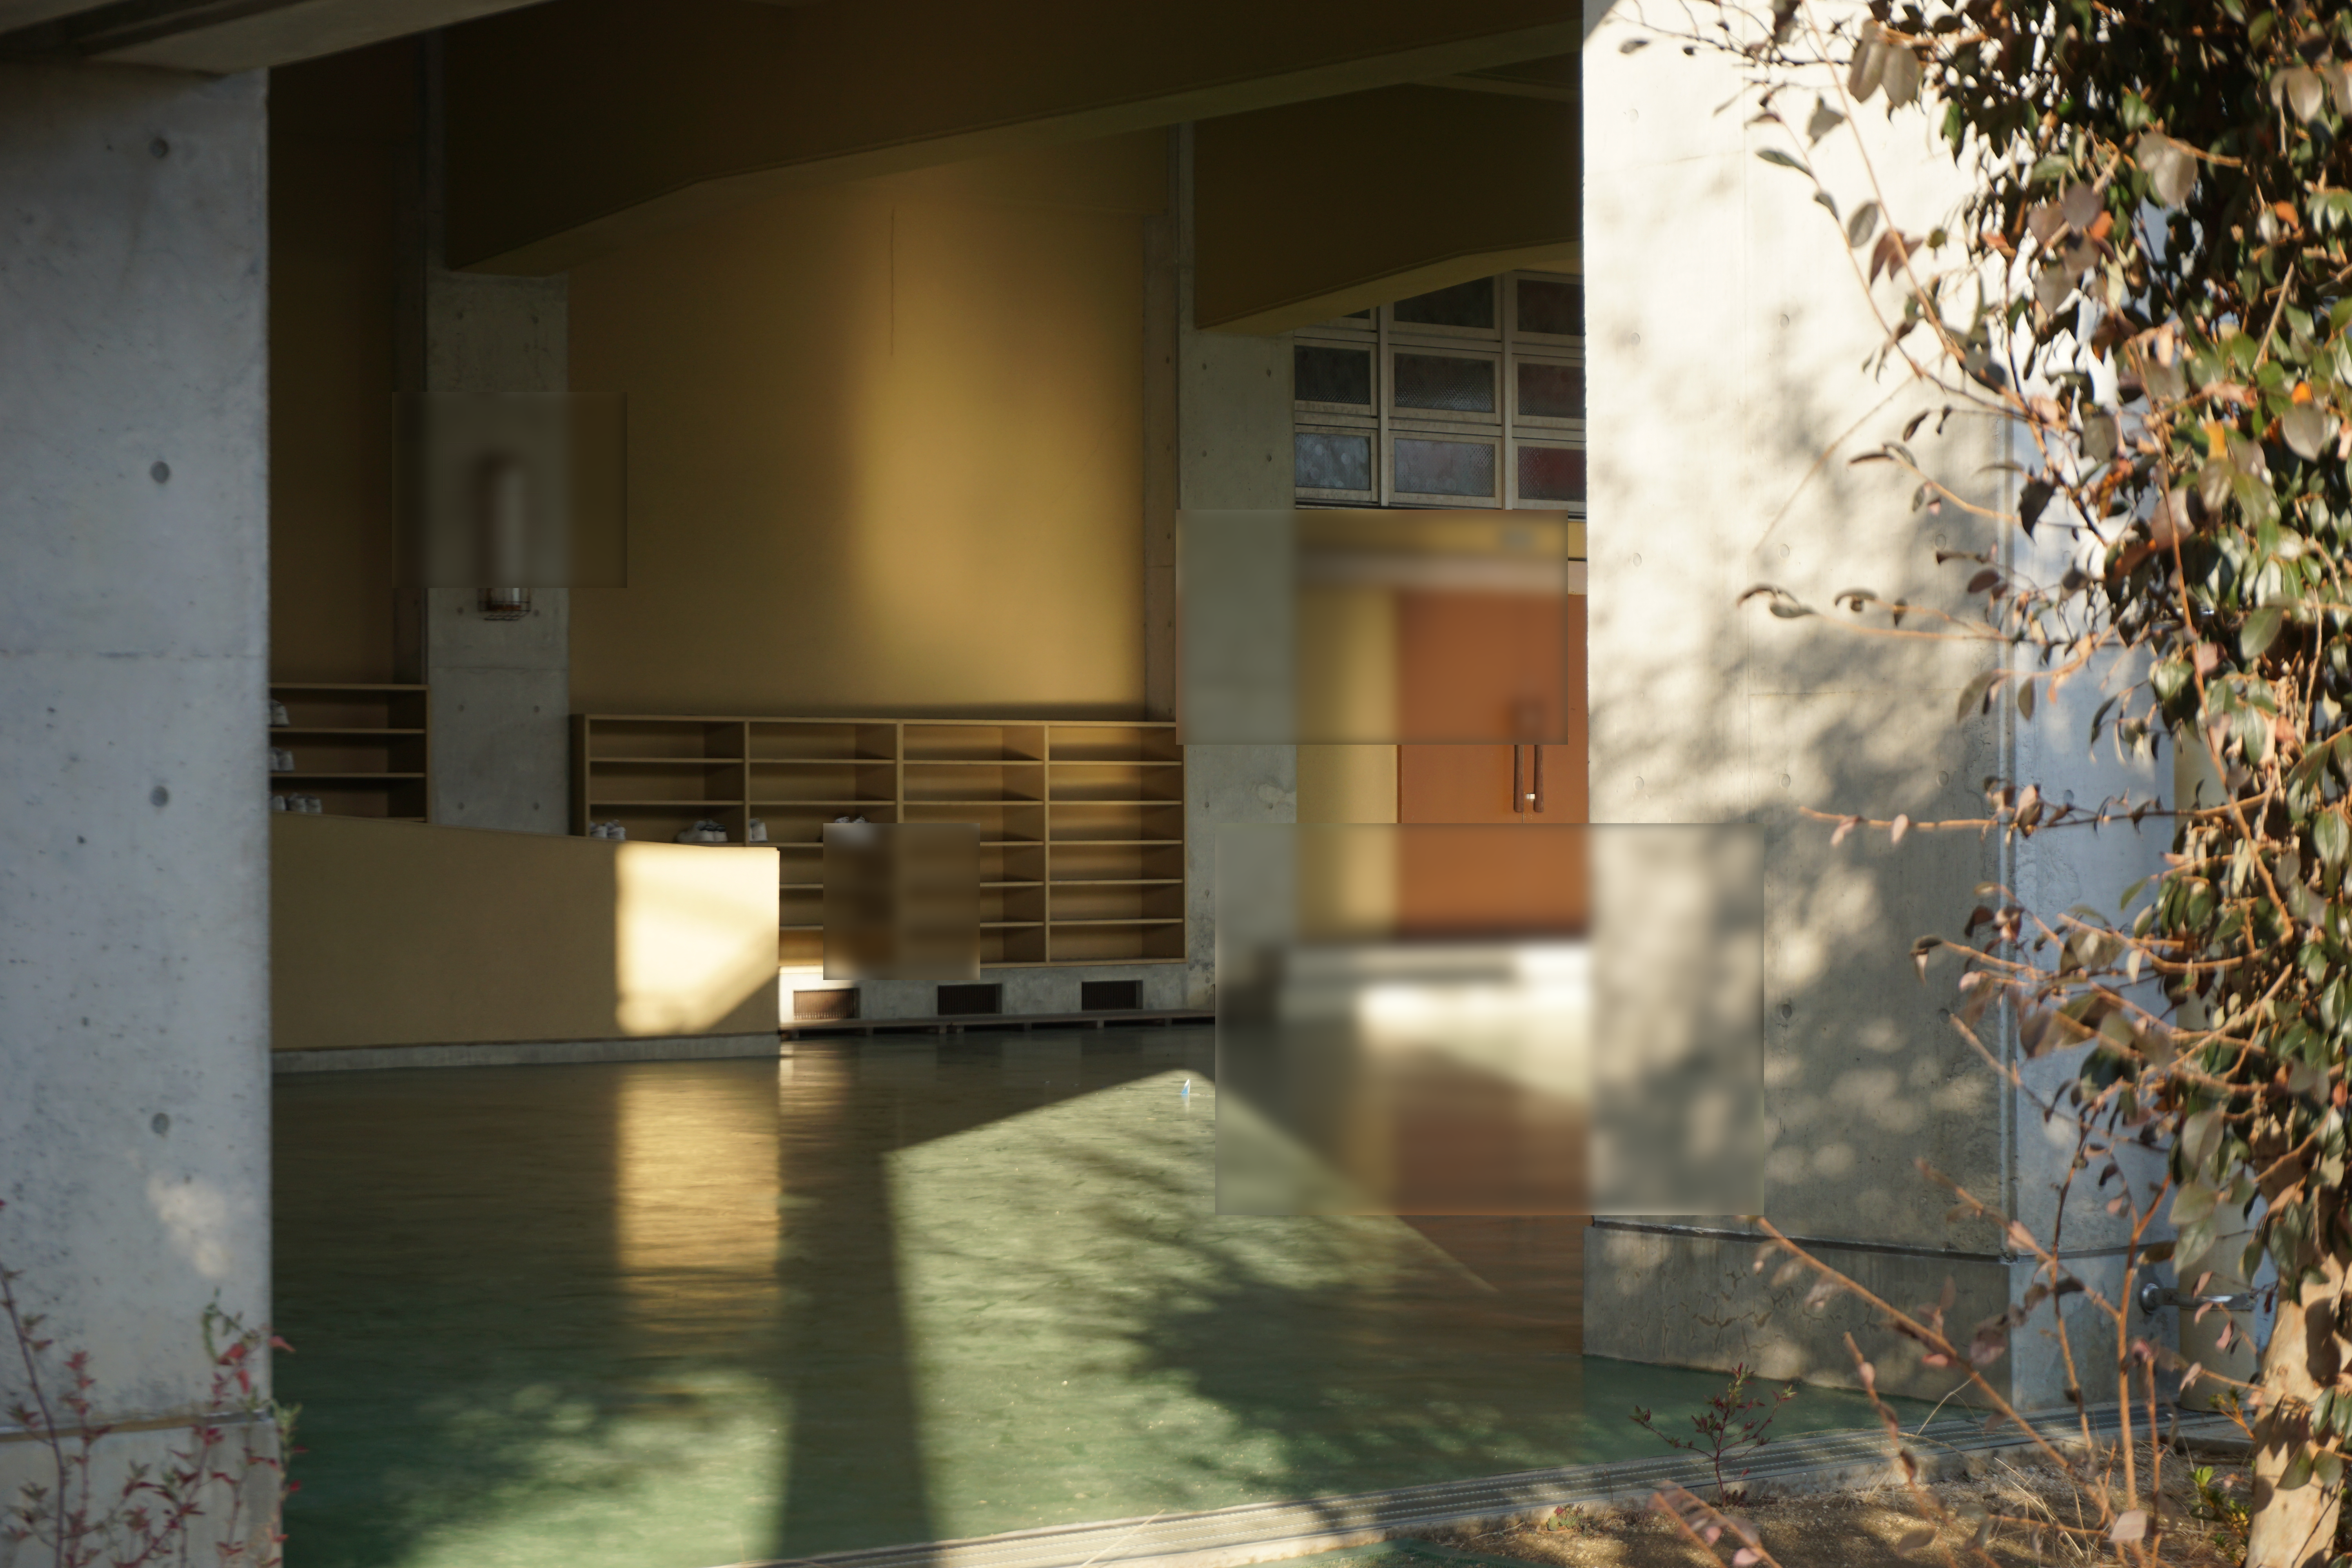
\includegraphics[width=1.0\textwidth]{pres_images/img05-de-blurred-blocks-result.png}
    \caption{de-blurred patches}
  \end{subfigure}
  
  \caption{sanity check on algorithm deblurring quality}
  \label{fig:2}
\end{figure}

Anyway, as I had a project to complete and with everything in place, I ran my program.
I calculated a bound for the number of samples for patches, created a rectangle, portioned
off that region in the image, passed into the blur-de-blur teams algorithm, and put the
resulting deblurred patch back into it's original place. When I ran it the lower bound
number of times, it took about 4 minutes. When I ran it the covering bound number of
times it took about 1.5 hours. Extrapolating, if I ran it for an upper bound number of
times, it would have taken 42 days. Astonishing!


\begin{figure}[!ht]
  \centering
  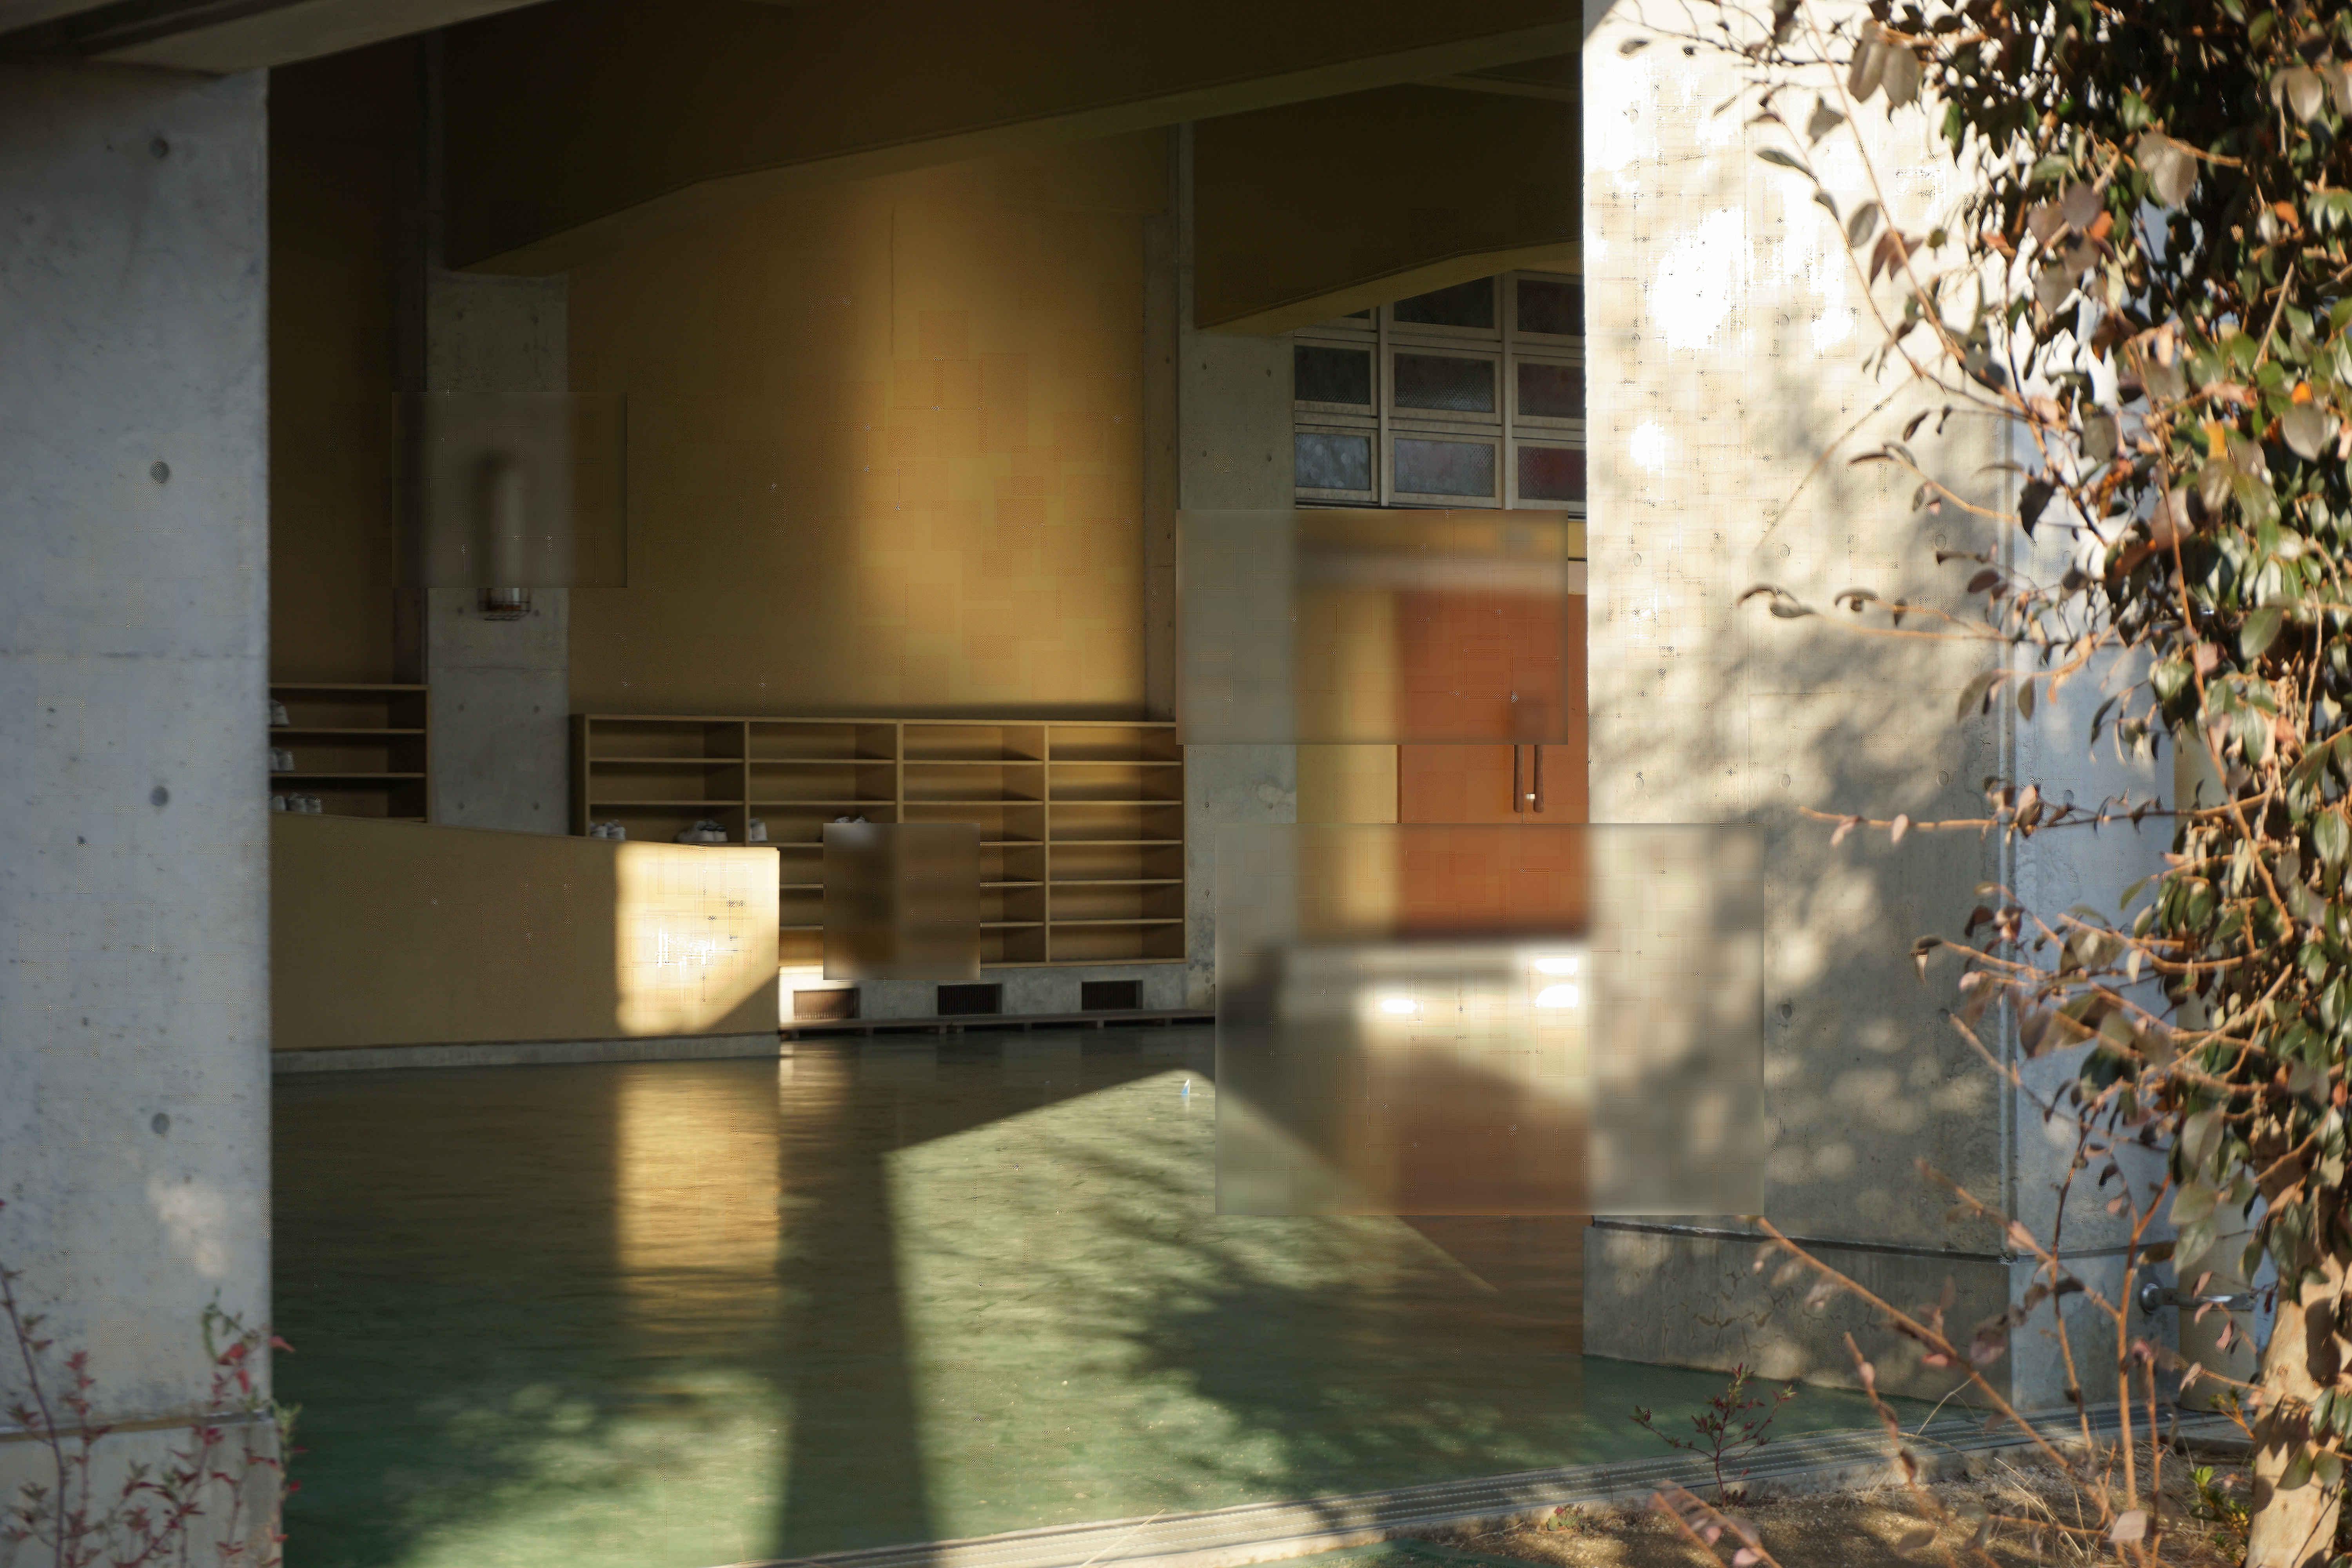
\includegraphics[width=1.0\textwidth]{pres_images/img06-de-blurred-covering.png}
  \caption{covering bound de-blurred image}
  \label{fig:3}
\end{figure}

One can see artifacts from the algorithm, and at least to me it appears regions with blur
were targeted more than other regions.

\subsection*{summary}

In summary I learned how cool the fourier transform is. I learned how the laplacian can
be used for edge detection. And I applied probability in a way that certainly improved
runtime.

%%%%%%%%%%%%%%%%%%%%%%%%%%%%%%%%%%%

% clear page for images to position where desired
\clearpage

%%%%%%%%%%%%%%%%%%%%%%%%%%%%%%%%%%%

\end{document}
